
%%%%%%%%%%%%%%%%%%%%%%% file typeinst.tex %%%%%%%%%%%%%%%%%%%%%%%%%
%
% This is the LaTeX source for the instructions to authors using
% the LaTeX document class 'llncs.cls' for contributions to
% the Lecture Notes in Computer Sciences series.
% http://www.springer.com/lncs Springer Heidelberg 2006/05/04
%
% It may be used as a template for your own input - copy it
% to a new file with a new name and use it as the basis
% for your article.
%
% NB: the document class 'llncs' has its own and detailed documentation, see
% ftp://ftp.springer.de/data/pubftp/pub/tex/latex/llncs/latex2e/llncsdoc.pdf
%
%%%%%%%%%%%%%%%%%%%%%%%%%%%%%%%%%%%%%%%%%%%%%%%%%%%%%%%%%%%%%%%%%%%


\documentclass[runningheads,a4paper]{llncs}

\usepackage{amssymb}
\setcounter{tocdepth}{3}
\usepackage{graphicx}
%\usepackage{multicol}
\usepackage{epstopdf}	
\usepackage{fancyvrb}
					% incluye eps, 1ro los pasa a PDF y luego lo incluye

\usepackage{url}
\urldef{\mailsa}\path|{jcaccav, spedre, pdecris, akatz, dbenders}@dc.uba.ar|
\newcommand{\keywords}[1]{\par\addvspace\baselineskip
\noindent\keywordname\enspace\ignorespaces#1}

\begin{document}

\hyphenation{re-latively}
\mainmatter  % start of an individual contribution

% first the title is needed
\title{\LARGE{A new programming interface for Educational Robotics}}

% a short form should be given in case it is too long for the running head
\titlerunning{Programming for Educational Robotics}

% the name(s) of the author(s) follow(s) next
%
% NB: Chinese authors should write their first names(s) in front of
% their surnames. This ensures that the names appear correctly in
% the running heads and the author index.
%
\author{Javier Caccavelli \and Sol Pedre\and Pablo de Crist\'oforis \and Andrea Katz \and Diego Bendersky}
%
\authorrunning{Programming for Educational Robotics}
% (feature abused for this document to repeat the title also on left hand pages)

% the affiliations are given next; don't give your e-mail address
% unless you accept that it will be published
\institute{Departamento de Computaci\'on,\\
Facultad de Ciencias Exactas y Naturales, \\
Universidad de Buenos Aires \\
Buenos Aires, Argentina\\
\mailsa}

%
% NB: a more complex sample for affiliations and the mapping to the
% corresponding authors can be found in the file "llncs.dem"
% (search for the string "\mainmatter" where a contribution starts).
% "llncs.dem" accompanies the document class "llncs.cls".
%

\maketitle


\begin{abstract}
%Educational Robotics uses robotics as a teaching tool in middle and high schools, and undergraduate curricula. %and popularization of science. The goal is to use robotics for teaching a variety of subjects other than specifically robotics. To achieve this goal is vital to have an adequate interface that allows unexperienced students to interact with robots in an easy manner. In this paper we present the current development of ERBPI (\emph{Easy Robot Behaviour Programmign Interface}), a new application that doesn't require any previous programming experience to control robots. To accomplish this, we propose to abandon the imperative programming paradigm and take a behaviour-based approach. Thus, the new application is based on the connectionist paradigm. The idea is to program the behaviors of robots by establishing connections between its sensors and actuators. This connections may include different mathematical functions, making it possible to achieve complex behaviours. Moreover, different defined behaviours can be connected using a subsumission architecture. The new application is designed to work with a variety of real robots and simulators, and it is designed so that adding new robots and simulators is easy. Learning experiences with high school students allowed us to test its effectiveness.

Educational Robotics uses robots as a tool for teaching a variety of subjects other than specifically robotics in undergraduate curricula. %middle and high schools.  
To achieve this goal is vital to have an adequate interface that allows inexperienced students to interact with robots in an easy manner. In this paper we present the current development of ERBPI (\emph{Easy Robot Behaviour Programming Interface}), a new application that doesn't require any previous programming experience to control robots. To accomplish this, we propose to abandon the imperative programming paradigm and take a behaviour-based approach. Thus, the new application is based on the connectionist paradigm, accomplishing behaviours by establishing configurable connections between sensors and actuators. Moreover, different defined behaviours can be connected using a subsumption architecture. The new application is designed to work with different robots and simulators, and it is simple for adding new ones. Learning experiences with high school students allowed us to test its effectiveness.

%comentario sol: me parece que hablar de paradigma conexionista es demasiado... mas bien creo q no existe. 
\keywords{educational robotics, behaviour-based programming interface.}
\end{abstract}


\section{Introduction}
\label{sec:intro}

The use of robots in undergraduate curricula has grown over the last years. The availability of low cost, easy-to-use platforms has even led to the use of robots in middle and high schools. Many teachers have an interest in introducing robots into their classrooms for teaching a variety of subjects other than specifically robotics. Thus, Educational Robotics arises, proposing the use of robotics as a teaching resource that allows inexperienced students to approach different scientific fields such as mathematics, experimental sciences, technology, information science and computing, among others. One of the aims of Educational Robotics is to aid students in building their own representations and concepts of science and technology, through the use, handling and control of robotic environments. This approach uses the constructionist process of designing, building, programming and debugging robot's behaviours, as well as collaboration and teamwork, as powerful means of enlivening education. 
%***citas del paper de Aibo [2, 6, 7]**** ver bien el afano de citas en este parrafo del primer parrafo de ambos papers.

Several educational robotics programming interfaces have been presented. Most are designed for university-level or late high school students and are implemented as extensions to existing programming languages. That is the case of Pyro \cite{pyro}, a Python-based programming framework which provides a set of abstractions that allow students to write platform-independent robot programs. Other interfaces include Not-Quite C (NQC) \cite{nqc} based on C, BrickOS \cite{brickos} based on C++ and leJOS \cite{lejos} that is based on Java. These three interfaces are particular for Lego Mindstrom. All these interfaces require programming experience or interest in learning a particular programming language. This makes them unsuitable for middle or high school students that do not handle any imperative or procedural programming concepts, such as the idea of loops, conditions, forks or variables in a program. %Educational Robotics courses, which aim at teaching subjects other than robotics or programming. 
Microsoft also offers the commercial tool Microsoft Robotics Developer Studio \cite{mrds}. This includes a visual programming interface based on a data flow approach, but again it requires knowledge of programming concepts, making it quite complex for inexperienced users. 

There are also several graphical environments for simulated robots aimed at middle schools. That is the case of StartLogo \cite{startlogo}, Squeak Etoys \cite{etoys} and Scratch \cite{scratch}. These are easy-to-use programming interfaces, allowing inexperienced students to make a quick start, although they maintain an imperative programming influence and are designed only for particular simulated environments. Another programming interface used in instructional settings at the K-12 level is RoboLab \cite{robolab} for the LEGO Mindstorms robot. This is a graphical environment in which students are given palettes of icons that they can drag and drop on a canvas. The icons represent robot components like motors and sensors, as well as abstract programming structures such as loops and counter variables. This interface is particular for the Mindstrom robot, and once again uses imperative programming structures that add complexity to the robotic environment. Finally, in \cite{robolab-ext} authors present an extension to RoboLab in order to work with other robotic platforms. 

%There are many works describing programming interfaces for Educational Robotics ***citas papers que presenten interfaces ***. Many of them emphasize the proposed applications as didactic tools, easy to learn and use for unexperienced public. To our knowledge, all involve the use of the imperative paradigm in some way for programming robots, . It is not clear if these applications are really easy to use for users that do not handle any imperative or procedural programming concepts, such as the idea of cycles, conditions or forks in a program.

Our experiences working with classroom teachers and young students have raised several issues that have motivated us to pursue the development of a behaviour-based interface, which abstracts away the imperative programming constructs and the low-level motor and sensor commands that often confuse inexperienced programmers or deter techno-phobic students. To accomplish this, we propose to abandon the imperative programming paradigm and take a behaviour-based approach. Thus, the proposed interface is based on a connectionist paradigm. The idea is that stimuli captured by the robot sensors are processed in a network of connections and result in a response for the robot actuators. To program the robot behaviours we have to establish connections between its sensors and actuators. This connections may include different mathematical functions \cite{braitenberg}. Moreover, different defined behaviours can be connected using a subsumption architecture \cite{subsumicion}, making it possible to achieve more complex behaviours. In this way, we get a state automaton (or machine), where each state represents a behaviour and each transition a change in the environment. This state machine can be easily translated into an imperative program that the robot executes to perform the behaviour.

This paper describes the current development of ERBPI(\emph{Easy Robot Behaviour Programming Interface}), a behaviour-based, easy to use robotic programming interface for Educational Robotics that allows to program different robotic platforms and simulators. The design of ERBPI follows the next criteria:

\begin{itemize}
\item \emph{Ease of use:} The user is not supposed to have any previous programming knowledge. The interface must be intuitive and easy to learn, providing all the tools to program robot behaviours graphically, making it possible to perform drag-and-drop with robot's sensors and actuators, build sensor-actuator connections, and easily configure them. 

\item \emph{Platform independence:} The application must work with a variety of robots and simulators, and be easily expandable to control new ones. The different bodies, sensors, actuators, low-level commands and protocols to communicate with high-level systems of different robots must be abstracted. Moreover, users must be able to test and run the same behaviours on multiple robots.

%\item \emph{Expressive power:} The application has to have a computing capacity similar to that provided by programming languages based on the imperative paradigm. This is necessary to perform complex robot behaviours. Our application use a connectionist paradigm to buid basic behaviours and subsumition architecture to build an automaton of state to interconnect them, making possible to achieve more complex behaviours. %(Comentario de Pablo: hasta que no tengamos una demostración formal de que lo que creamos es Turing Compatible no podemos afirmar que tenemos un poder de expresividad equivalente a los programas imperativos. Por eso puse la palabra "similar". Para mi, si en algún momento hacemos esta demostración tenemos un paper para una revista!)
%\item \emph{Comprehensive expressive power:} VER Q PONER ACA - FALTA

%\item \emph{Good for testing and debbuging environment:} PONEMOS ALGO DE LA IDEA DEL DEBUG Y TESTING CON LA WEBCAM? - FALTA (Comentario de Pablo: El problema es que no sabemos si esto realmente se va a poder hacer y no tenemos nada hecho de esto. Yo de la cámara no pondría nada).

\item \emph{Portability:} The application must work in different operating systems and platforms to accommodate the different hardware and software available in schools or other educational institutions.  

\item \emph{Flexibility:} Students from a wide range of backgrounds and teachers with a broad range of goals must be able to use the programming interface effectively, accommodating different levels, curricular needs, academic subjects and physical environments for instruction.

\end{itemize}

This paper is organized as follows. In the next section we describe ERPBI's architecture and features, and give examples of use. Afterward, we comment some experiences using ERPBI in the classroom with high school students. Finally, we draw some conclusions and discuss directions for future work.


\section{The ERBPI: Easy Robot Behaviour Programming Interface}
\label{sec:erbpi}
%%%%%%%%%%%%%%%%%%%%%%%%%%%%%%%%%%%%%%%%%%%%%%%%%%%%%%%%%%%%
%% ERBPI
%%%%%%%%%%%%%%%%%%%%%%%%%%%%%%%%%%%%%%%%%%%%%%%%%%%%%%%%%%%%


La idea general del software es que permita, a trav�s de una interfaz gr�fica y sencilla,
programar los robots para realizar distintas experiencias de veh�culos de Braitenberg y 
comportamiento basado en subsumisi�n\footnote{\textit{Subsumption Architecture}, Behavior-Based Robotics, R. C. Arkin.}.

Para eso, nos basamos en el survey que realizamos, principalmente los programas \textit{StarLogo} y \textit{Scratch}, 
que resultaron los mejorcitos en cuanto a la interfaz gr�fica de programaci�n y la idea de la interfaz gr�fica de proveer menus y submen�es con los objetos predefinidos para ir agregando...

La idea es poder combinar \textit{Braitenberg} y \textit{Subsumisi�n}, de manera que cada estado de la maquina de estados de subsimisi�n sea un braitenberg.
Entonces, en principio, se puede hacer s�lo Braitenberg. Luego, se puede hacer Subsumisi�n ``insertando'' en cada estado un braitenberg 
definido anteriormente.

Algo as� como la Figura \ref{Fig:subsumision}:

\begin{figure}
	\centering
	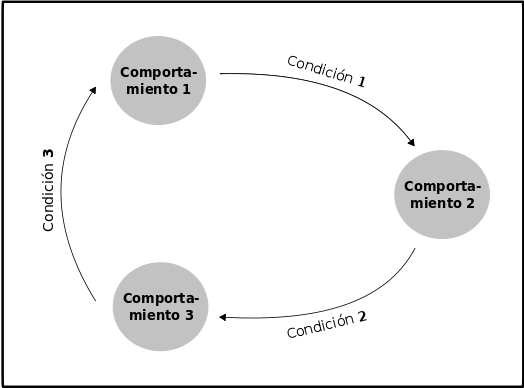
\includegraphics[scale=0.7]{images/subsumision.png}
	\caption{FORMA GENERAL DISE\~nO SOFTWARE.}
	\label{Fig:subsumision}
\end{figure}

ARREGLAR ESTO, COMPLETAR CON LO DEL EUROBOT2011 QUE EST\'A MUY BIEN...

\section{ERBPI in the classroom}
\label{sec:experiments}
%ERBPI's goal is to provide an easy interface that allows inexperienced students to interact with robots, thus providing a tool for Educational Robotics courses in schools. 
To explore the adequacy of the tool, a preliminary version of ERBPI was used in a special course designed for high school students during July 2010. 

The class was composed of 20 students from seven %technical (Comentario Pablo: yo sacaría que fueron escuelas técnicas porque toda la justificación era que la aplicación estaba dirigida a estudiantes que no sabían programar) 
high schools of Buenos Aires, Argentina. The student's programming experience varied from none to some experience with procedural languages like C, C++ or Pascal. There were also few students with some electronics background, and all mastered basic mathematical concepts such as constant, monotonous and broken functions. None of the students had experience with robots. 

The course covered basic concepts of robotics and of behaviour based robotics. The preliminary version of ERBPI used for the course only had the basic conectionnist approach, lacking the subsumption feature to compose more complex behaviours. We followed a hands-on approach, programming easy behaviours from day one in groups of two or three students. Using the Braitenberg model \cite{braitenberg}, the students developed behaviours in simulators that were also tested in real robots, experiencing with the Yaks simulator \cite{yaks}, Khepera \cite{khepera} and ExaBot \cite{exabot} robots. 
Different behaviours were proposed for the students to solve with the robots, ranging from follow a line in the floor, go to a light spot, avoid obstacles or solve mazes.
Those behaviours were developed by teaching students the scientific method, encouraging them to propose hypothesis, contrast the expected results with the ones obtained in the testing phase, and then propose explanations and changes to the original robot control. Each group also shared their findings with the rest of the class, showing different approaches and solutions to the given problems during a discussion phase. Overall, the students picked up the use of ERBPI easily and could program all the proposed behaviours quickly. %They also applied the base of the scientific method in their experiences naturally. 

After the course, a questionnaire was given to the students in order to explore their reviews of the course and the programming interface. All students answered that they had found the interface easy to learn and use, despite they had no idea about programming robots and had not had the opportunity to control a robot before the course. All students felt that they met the objectives of the course successfully and most of them showed interest in taking more courses of robotics, computer science and engineering after the course. 

In this experience we found some improvements to be made in ERBPI. For example, we plan to execute the resulting program directly in the robot when possible, instead of executing the program in the external PC with the consequent transmission of sensor data and commands back and forth. Another improvement is to increase the amount of possible functions, to broaden the tools capabilities for math teachers. We also realized how important the subsumption architecture feature is, to allow the construction of more complex behaviours from simpler ones. Students also suggested some improvements, like ``cooler'' or friendlier names for different objects of ERBPI. %(i.e. to call the constant speed functions for the motors ``power balls''). 

We also tested ERBPI in shorter courses, lectures, exhibitions and others activities of popularization of science for high school students and broader public. The most important was part of a three day exhibition of the University of Buenos Aires that took place in October 2010 \cite{expouba}. Many of the ideas in ERBPI were born in previous experiences with high school students, mainly two eight-week workshop on robotics we organized as a part of a program from the Vocational Orientation Department of our Faculty during 2006 \cite{taller2006} and 2009 \cite{taller2009}. 

We are planning on using a full featured ERBPI in Educational Robotics courses for more high schools of Buenos Aires during the present year, as a part of a popularization of science project of our Faculty. 

\section{Conclusions and ongoing work}
\label{sec:conclusion}
In this paper we presented the design and current development of ERBPI, an application to provide a simple, graphical, behaviour-based interface for Educational Robotics courses aimed at inexperienced students. To reach this goal, we propose to abandon the imperative paradigm and take a behaviour based approach. The tool is capable of controlling different robotics platforms, and it is designed to be easily expandable for new ones. It is also portable to different operating systems to accommodate the available hardware and software in schools. Experiences with high school students show that the current version of ERBPI allows inexperienced public to quickly start working with robotic environments. 

We are currently working on the subsumption feature of the tool, important to allow the development of more complex behaviours. We also plan to expand the application in order to execute the behaviour directly on the robot when possible. Another improvement we are working on is to include a play-back facility to debug behaviours, using the execution log-file and a web-cam that films the robot behaviour. The idea is to use the execution log-file to show at the same time which sensors, connections and behaviours were activated when the robot took a certain action, and the play-back of the video captured with the web-cam. 

During the present year we will prepare and teach educational robotics courses for more high schools in Buenos Aires, using the full featured ERBPI tool. We hope this experiences will provide extra feedback to continue and improve this project. 




\begin{thebibliography}{19}


%\bibitem{}E. Sklar, S. Parsons, and P. Stone. Using RoboCup in university-level computer science education. Journal on Educational Resources in Computing (JERIC), Special Issue on robotics in undergraduate education, part I, 4(2), September 2004

\bibitem{pyro} D.S. Blank, D. Kumar, L. Meeden, and H. Yanco. Pyro: A python-based versatile programming environment for teaching robotics. Journal on Educational Resources in Computing(JERIC), Special issue on robotics in undergraduate education. Part 2, 4(3):115, 2004.

\bibitem{nqc} Baum. NQC. http://bricxcc.sourceforge.net/nqc/, accessed March 17, 2011.

\bibitem{brickos} Markus. brickOS. http://brickos.sourceforge.net/, accessed March 17, 2011.

\bibitem{lejos} J. Solorzano. leJOS. http://lejos.sourceforge.net/, accessed March 17, 2011.

\bibitem{mrds} Microsoft Robotics Developer Studio, http://www.microsoft.com/robotics/, accessed March 17, 2011.

\bibitem{startlogo} MIT's Scheller Teacher Education Program (STEP), http://education.mit.edu/ drupal/starlogo-tng, accessed March 17, 2011.

\bibitem{etoys} http://www.squeakland.org/, accessed March 17, 2011.

\bibitem{scratch} http://scratch.mit.edu/, accessed March 17, 2011.

\bibitem{robolab} Tufts University. RoboLab. http://www.ceeo.tufts.edu/robolabatceeo/, accessed March 17, 2011.

\bibitem{robolab-ext} M. Q. Azhar, An agent-oriented behavior-based interface framework for educationa robotics, In Agent-Based Systems for Human Learning (ABSHL) Workshop at Autonomous Agents and MultiAgent Systems (AAMAS-2006),2006.

\bibitem{braitenberg} V. Braitenberg, Vehicles: Experiments in Synthetic Psychology, MIT Press, Cambridge, 1986.

\bibitem{subsumicion} R. C. Arkin, Behavior-Based Robotics, MIT Press, Cambridge, 1998.

\bibitem{topologicalSorting}  H. Cormen, C. E. Leiserson, R. L. Rivest, C. Stein, Topological Sort, Introduction to Algorithms, MIT Press, Cambridge, 2009.

\bibitem{khepera} K-Team, Khepera I, http://www.k-team.com/, accessed March 17, 2011. 

\bibitem{exabot} Sol Pedre, Pablo de Cristóforis, Javier Caccavelli and Andrés Stoliar, A mobile mini robot architecture for research, education and popularization of science, Journal of Applied Computer Science Methods, Guest Editors: Jacek Zurada and Pablo Estevez, vol 2, no 1 pp 41-59, ISSN 1689-9636. 

\bibitem{yaks} Yet Another Khepera Simulator, http://freshmeat.net/projects/yaks/, accessed March 17, 2011. 

\bibitem{player} Player/Stage Simulator, http://playerstage.sourceforge.net/, accessed March 17, 2011.
%\bibitem{talleres} Science workshops, http://www.fcen.uba.ar/dov/talleres_de_ciencia/TALLERES_de_ciencia.htm, accessed March 17, 2011. 
\bibitem{expouba} ExpoUBA 2010, Plaza de las Ciencias, Universidad de Buenos Aires, Argentina, http://www.uba.ar/expouba, accessed March 17, 2010. %http://exactas.uba.ar/institucional/display.php?estructura=1\&desarrollo=0\&id\_caja=238\&nivel\_caja=2

\bibitem{taller2006} Robot programming workshop for high school students, www.fcen.uba.ar /dov/talleres\_de\_ciencia/2006/computacion.htm, accessed March 17, 2011. 

\bibitem{taller2009} Robot programming workshop for high school students, www.fcen.uba.ar /dov/talleres\_de\_ciencia/2009/computacion.htm, accessed March 17, 2011.

\end{thebibliography}

\end{document}
